% Options for packages loaded elsewhere
\PassOptionsToPackage{unicode}{hyperref}
\PassOptionsToPackage{hyphens}{url}
%
\documentclass[
]{article}
\usepackage{amsmath,amssymb}
\usepackage{iftex}
\ifPDFTeX
  \usepackage[T1]{fontenc}
  \usepackage[utf8]{inputenc}
  \usepackage{textcomp} % provide euro and other symbols
\else % if luatex or xetex
  \usepackage{unicode-math} % this also loads fontspec
  \defaultfontfeatures{Scale=MatchLowercase}
  \defaultfontfeatures[\rmfamily]{Ligatures=TeX,Scale=1}
\fi
\usepackage{lmodern}
\ifPDFTeX\else
  % xetex/luatex font selection
\fi
% Use upquote if available, for straight quotes in verbatim environments
\IfFileExists{upquote.sty}{\usepackage{upquote}}{}
\IfFileExists{microtype.sty}{% use microtype if available
  \usepackage[]{microtype}
  \UseMicrotypeSet[protrusion]{basicmath} % disable protrusion for tt fonts
}{}
\makeatletter
\@ifundefined{KOMAClassName}{% if non-KOMA class
  \IfFileExists{parskip.sty}{%
    \usepackage{parskip}
  }{% else
    \setlength{\parindent}{0pt}
    \setlength{\parskip}{6pt plus 2pt minus 1pt}}
}{% if KOMA class
  \KOMAoptions{parskip=half}}
\makeatother
\usepackage{xcolor}
\usepackage[margin=1in]{geometry}
\usepackage{longtable,booktabs,array}
\usepackage{calc} % for calculating minipage widths
% Correct order of tables after \paragraph or \subparagraph
\usepackage{etoolbox}
\makeatletter
\patchcmd\longtable{\par}{\if@noskipsec\mbox{}\fi\par}{}{}
\makeatother
% Allow footnotes in longtable head/foot
\IfFileExists{footnotehyper.sty}{\usepackage{footnotehyper}}{\usepackage{footnote}}
\makesavenoteenv{longtable}
\usepackage{graphicx}
\makeatletter
\def\maxwidth{\ifdim\Gin@nat@width>\linewidth\linewidth\else\Gin@nat@width\fi}
\def\maxheight{\ifdim\Gin@nat@height>\textheight\textheight\else\Gin@nat@height\fi}
\makeatother
% Scale images if necessary, so that they will not overflow the page
% margins by default, and it is still possible to overwrite the defaults
% using explicit options in \includegraphics[width, height, ...]{}
\setkeys{Gin}{width=\maxwidth,height=\maxheight,keepaspectratio}
% Set default figure placement to htbp
\makeatletter
\def\fps@figure{htbp}
\makeatother
\setlength{\emergencystretch}{3em} % prevent overfull lines
\providecommand{\tightlist}{%
  \setlength{\itemsep}{0pt}\setlength{\parskip}{0pt}}
\setcounter{secnumdepth}{-\maxdimen} % remove section numbering
\newlength{\cslhangindent}
\setlength{\cslhangindent}{1.5em}
\newlength{\csllabelwidth}
\setlength{\csllabelwidth}{3em}
\newlength{\cslentryspacingunit} % times entry-spacing
\setlength{\cslentryspacingunit}{\parskip}
\newenvironment{CSLReferences}[2] % #1 hanging-ident, #2 entry spacing
 {% don't indent paragraphs
  \setlength{\parindent}{0pt}
  % turn on hanging indent if param 1 is 1
  \ifodd #1
  \let\oldpar\par
  \def\par{\hangindent=\cslhangindent\oldpar}
  \fi
  % set entry spacing
  \setlength{\parskip}{#2\cslentryspacingunit}
 }%
 {}
\usepackage{calc}
\newcommand{\CSLBlock}[1]{#1\hfill\break}
\newcommand{\CSLLeftMargin}[1]{\parbox[t]{\csllabelwidth}{#1}}
\newcommand{\CSLRightInline}[1]{\parbox[t]{\linewidth - \csllabelwidth}{#1}\break}
\newcommand{\CSLIndent}[1]{\hspace{\cslhangindent}#1}
\ifLuaTeX
  \usepackage{selnolig}  % disable illegal ligatures
\fi
\IfFileExists{bookmark.sty}{\usepackage{bookmark}}{\usepackage{hyperref}}
\IfFileExists{xurl.sty}{\usepackage{xurl}}{} % add URL line breaks if available
\urlstyle{same}
\hypersetup{
  pdftitle={CSC8639 Interim Report: Explaining Time Series Downsampling},
  pdfauthor={Author: 210431461 \textbar{} Supervisor: Matthew Forshaw},
  hidelinks,
  pdfcreator={LaTeX via pandoc}}

\title{CSC8639 Interim Report: Explaining Time Series Downsampling}
\author{Author: 210431461 \textbar{} Supervisor: Matthew Forshaw}
\date{}

\begin{document}
\maketitle

\hypertarget{introduction}{%
\subsubsection{Introduction}\label{introduction}}

Decision-makers must trust that the data being considered sufficiently
represents the situation they are deciding on. Trusting the data means
trusting which data points are selected, how this data collected and
stored, and the capability of data practitioners to understand the
quality, insights and limitations of it. This data pipeline can obscure
or loose important information making it difficult to determine and
explain that the data reliably and truthfully reflects the situation in
question. Today's increasing volume of data makes this even more
difficult (Yanzhe An and Wang (2022)).

This problem is particularly pertinent to collections of observations
obtained through repeated measurements over time (Statistics (2023)),
known as time series data. ``{[}W{]}idely generated by industry and
research at an increasing speed'' (Yanzhe An and Wang (2022)),
voluminous time series data is putting unprecedented demand on resources
(Schlossnagle, Sheehy, and McCubbin (2021), Atlam, Walters, and Wills
(2018)). This is forcing data practitioners to utilise methods, such as
aggregation, windowing, and downsampling, that reduce data volumes to
align with cost or time limitations, storage capabilities, and
sustainability ambitions (Steinarsson (2013), Yanzhe An and Wang (2022),
Tank (2020)). These reduction methods involve discarding data, which
could result in the further loss of important information for
decision-makers, and reduce the representativeness of the data.

However, discarding this data is a vital part of making voluminous time
series understandable for human observation (Steinarsson (2013)).
Downsampling reduces ``\ldots the number of data points while preserving
the overall shape of the time series'' (Donckt et al. (2023)), allowing
the human eye to observe only the most valuable data points. Line graphs
are an effective and popular method for visualising this data (Yunhai
Wang and Yu (2023)). Despite effectively conveying the overall shape of
the time series data (Aigner et al. (2008)), they offer little insight
into which downsampling approach and parameters best represent the
original data. Better visualising the impact of downsampling time series
data, is likely help data practitioners confidently select their
downsampling approach and better explain the insights and limitations of
downsampled data. In doing so, data practitioners can better support
decision-makers to trust the data they are considering.

\hypertarget{aim-and-objectives}{%
\subsubsection{Aim and Objectives}\label{aim-and-objectives}}

The research outlined by this interim report aims to improve how data
practitioners better understand and explain the impact of downsampling
time series data. It is hoped that this research will support data
practitioners to determine and communicate whether data being considered
by decision-makers reliably and truthfully reflects the situation in
question, and help increase decision-makers trust in data-led
decision-making.

To better understand and explain the impact of downsampling voluminous
time series data, the research addresses the following five objectives:

\begin{itemize}
\item
  Develop a baseline understanding current downsampling algorithms'
  impact on original data sets by using the R package \texttt{ImputeTS}
  (Moritz and Bartiz-Beielstein (2017)) to compare visualisations of the
  original and compressed data.
\item
  Conduct exploratory analysis to determine common properties of time
  series data, attempting to refine the 22 time series features
  identified by \texttt{catch22} (Lubba et al. (2022)) to identify the
  most useful features for comparing the impacts of downsampling
  algorithms on original time series data.
\item
  Design comparative visualisations of the most useful features of time
  series data across different downsampling algorithms to help
  communicate their impacts on the original data.
\item
  Survey existing metrics used to compare downsampled data
  representativeness to inform an evaluation method for this research.
\item
  Conduct user research with data practitioners and decision-makers to
  understand how they engage with downsampled time series data and its
  trustworthiness.
\end{itemize}

The aim and objectives set out here are ambitious; it is likely that
each objective could be an individual project and the author is a
part-time student. Given this, this project will delivered iteratively;
the research objectives will be continuously reviewed to successfully
deliver the most impact in the available time.

\hypertarget{project-plan}{%
\subsubsection{Project Plan}\label{project-plan}}

This project is divided in to five activity themes (Milestones, Reading,
Exploratory Data Analysis, Visualisation, User Research) and six phases
(1-6) to deliver the research aim and objectives by 15 August 2023. This
plan is visualised on the next page.

\textbf{Overview of Progress}

Progress on the project so far includes activity specified in phases (1)
and (2) as well as some phase (3) activities, where progress to date is
visualised as a percentage. Further details on this progress are set out
below by activity theme:

\begin{itemize}
\item
  \emph{Milestones:} Four meetings between the project supervisor and
  author have taken place, where the project scope, approach, aims and
  objectives have been clarified. A short title, description, and
  ethical approval have been submitted as required. The Data Management
  Plan is completed and shared in Annex A.
\item
  \emph{Reading:} Initial exploratory reading around time series data
  and downsampling was conducted before the supervisor recommended nine
  sources. These sources were read, and further reading of referenced
  sources is underway.
\item
  \emph{Exploratory Data Analysis:} The data sets for exploration were
  identified with support from the supervisor; the author has drafted
  questions to guide exploration and initial visual exploration is being
  conducted on selected data sets.
\item
  \emph{Visualisation:} Potential visuals for user research are being
  collated, but this activity theme is not a focus of phase (1) and (2).
\item
  \emph{User Research:} The approach to user research has been designed
  and discussed with the supervisor; invites, consent form,question
  list, and an initial list of participants are drafted. The invite,
  consent form, and question list are attached to this interim report
  (Annex B, C, and D).
\end{itemize}

\textbf{Overview of Project}

The visualisation of the project plan highlights the key activities
within each theme across the project phases. Because of this iterative
approach, it was agreed with the project supervisor that an agile
approach was appropriate; the project plan is visualised as an agile
roadmap. This visualisation, created on a platform provided by
\texttt{roadmunk}, is interactive and will be updated to reflect the
iterative nature of the project.

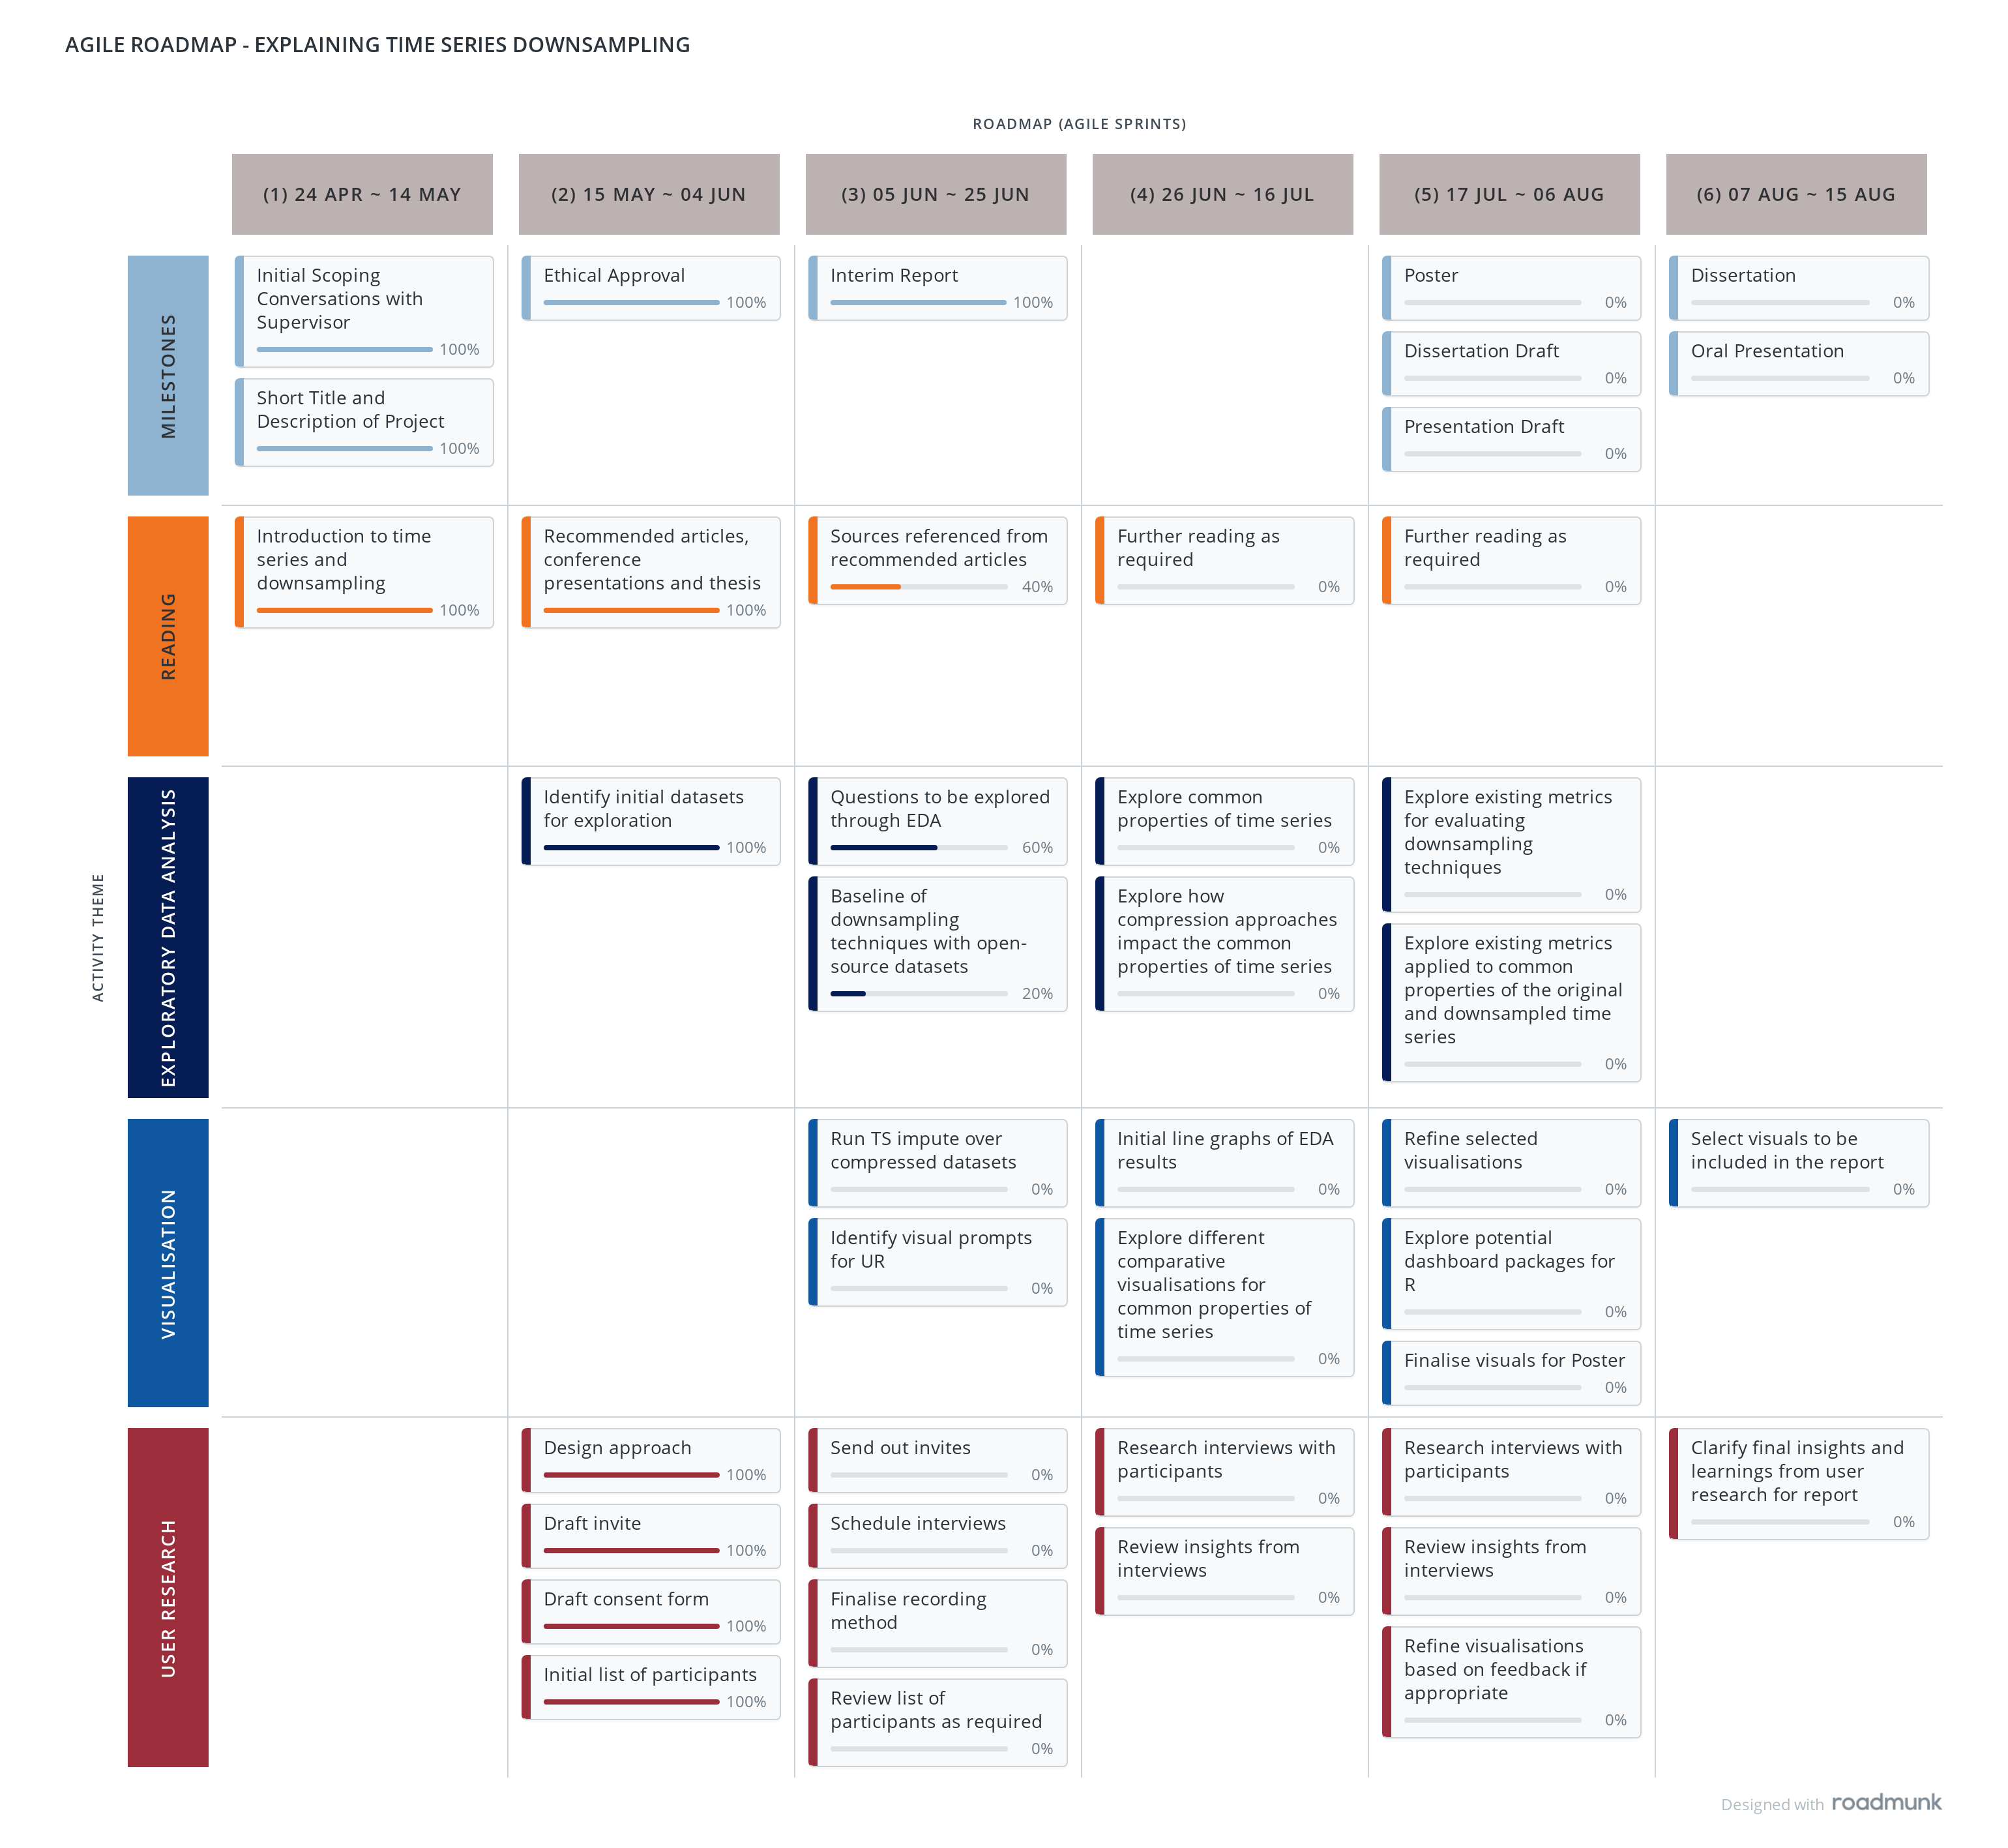
\includegraphics{D:/Morgan/Documents/NCL MSc/final_project/mofrod_project/docs/Agile Roadmap - Explaining Time Series Downsampling.png}

\newpage

\textbf{Project Risks and Mitigation}

To be delivered successfully, there are several risks that this project
may need to mitigate. These are set out in the table below with a risk
rating of low, medium or high.

\begin{longtable}[]{@{}
  >{\centering\arraybackslash}p{(\columnwidth - 6\tabcolsep) * \real{0.2432}}
  >{\centering\arraybackslash}p{(\columnwidth - 6\tabcolsep) * \real{0.2432}}
  >{\centering\arraybackslash}p{(\columnwidth - 6\tabcolsep) * \real{0.2162}}
  >{\centering\arraybackslash}p{(\columnwidth - 6\tabcolsep) * \real{0.2973}}@{}}
\toprule\noalign{}
\begin{minipage}[b]{\linewidth}\centering
\textbf{Impact}
\end{minipage} & \begin{minipage}[b]{\linewidth}\centering
\textbf{Likelihood}
\end{minipage} & \begin{minipage}[b]{\linewidth}\centering
\textbf{Risk}
\end{minipage} & \begin{minipage}[b]{\linewidth}\centering
\textbf{Mitigation}
\end{minipage} \\
\midrule\noalign{}
\endhead
\bottomrule\noalign{}
\endlastfoot
Low & High & Fewer people agreed to participate in User Research than
expected. & Invites will be sent in a phased approach to enable further
invites to be sent if response numbers are lower than expected. \\
------ & ------ & ------ & ------ \\
Low & High & Number of decision-makers and data practitioners who agreed
to participate in User Research is imbalanced. & The numbers for User
Research are unlikely to be statistically significant for this project
anyway, so any further limitations on the findings of User Research and
their impact will be set out in the final report. \\
------ & ------ & ------ & ------ \\
Low & Medium & Data availability and cleaning take a significant amount
of time, and may detract from original research. & A subs-selection of
open source data previous time series visualisation research has been
chosen in mitigation. \\
------ & ------ & ------ & ------ \\
Low & Medium & The outputs from User Research, such as interview content
or personal details, are not stored and treated securely. & Consent
forms will be collected prior to scheduling interviews and participants
will be annonymised in a locked spreadsheet saved separated from the
project. There will be no personal details associated with the interview
content, which will also be saved in a locked folder separate from the
project. \\
------ & ------ & ------ & ------ \\
Medium & Medium & There are several elements of this project that are,
to some extent, dependent on other project elements. For example, the
exploratory data analysis and visualisation. & These dependencies are
being mitigated by the agile approach to the project, allowing the
author to adapt as needed, and clear communication with the
supervisor. \\
------ & ------ & ------ & ------ \\
High & Medium & The author is a part-time student working towards the
same deadlines and criteria as full-time students. & The agile roadmap
clearly sets out how the project is likely to progress, and the research
objectives have been selected to help maximise impact if there are
delays with some components. Progress will be clearly communicated to
the supervisor, and an extension may be applied for if required. \\
\end{longtable}

This list of risks and mitigations will be reviewed and updated
throughout the project as more may arise when the research is iterated.

\hypertarget{conclusion}{%
\subsection{Conclusion}\label{conclusion}}

The research of this project aims to improve how data practitioners
better understand and explain the impact of downsampling time series
data. This report has introduced the research topic by outlining why
this matters, set out the research aim and objectives as well as
progress so far, visualised the project plan and explained the risks
that may need mitigated. The information provided in the report will be
continuously reviewed in consultation with the project supervisor so
that the research is delivers the most impact in the time available.

\newpage

\hypertarget{annex-a-data-management-plan}{%
\subsection{Annex A: Data Management
Plan}\label{annex-a-data-management-plan}}

\hypertarget{proposal-name}{%
\paragraph{0. Proposal name}\label{proposal-name}}

Explaining Time Series Downsampling

\hypertarget{description-of-the-data}{%
\paragraph{1. Description of the data}\label{description-of-the-data}}

\textbf{1.1 Type of study}

Improving how data practitioners better understand and explain the
impact of downsampling time series data, this study includes time series
data sets, exploratory analysis, of these datasets in R, user research
and comparative surveys of compression algorithms, common evaluation
metrics, and time series visualisations.

\textbf{1.2 Types of data}

Both quantitative data from open-source data sets and qualitative data
from user research will be used in this study.

The quantitative data sets are being sourced from the Alan Turing
Institute `AnnotateChange'
(\url{https://github.com/alan-turing-institute/AnnotateChange}) and
`Turing Change Point Dataset'
(\url{https://github.com/alan-turing-institute/TCPD/tree/master}). The
`AnnotateChange' repository was created to collect annotations of time
series data to construct the `Turing Change Point Dataset' repository by
Van den Burgh and Williams (2020). The publicly available data in these
datasets will be used within the stipulated licensing agreement(s)
stipulated by the data owner(s).

The qualitative data will be collected from interviews with
decision-makers and data practitioners.

\textbf{1.3 Format and scale of the data}

The qualitative data will be collected via recorded video calls with
participants and notes taken in csv files.

The quantitative demo data from `AnnotateChange' will be used initially
as JSON scripts are provided. A subset of data is likely to be selected
from the 'Turing Change Point Dataset', which includes 37 datasets of
time series data from a variety of contexts as well as 5 quality control
datasets. The data across these repositories are provided in different
formats pending where the original data is hosted. The FAIR principles
(Findability, Accessibility, Interoperability and Reusability) are
satisfied by the Alan Turin Institute's use of these datasets as
benchmark suites. The project will also utilise R, RStudio and a variety
of R packages, like RMarkdown to ensure reproducibility.

\hypertarget{data-collection-generation}{%
\paragraph{2. Data collection /
generation}\label{data-collection-generation}}

\textbf{2.1 Methodologies for data collection / generation}

No new time series data will be collected for this study. The results
created during this research will be clearly documented in the report,
tables and reproducible code housed in GitHub
(\url{https://github.com/MoFrod/downsampling_timeseries/tree/main}).

New data will be collected from interviews with data practitioners and
decision-makers considering time series data. There is no data source
that currently sets out the perspectives of these users, so new data is
needed. This new qualitative data will be collected from a standardised
list of interview questions that are asked to volunteer participants.

\textbf{2.2 Data quality and standards}

The quantitative data quality of the datasets is acceptable in line with
the FAIR principles, and data cleaning will be conducted as required.
The qualitative data quality cannot be determined until it is collected.

\hypertarget{data-management-documentation-and-curation}{%
\paragraph{3. Data management, documentation and
curation}\label{data-management-documentation-and-curation}}

\textbf{3.1 Managing, storing and curating data.}

The qualitative data generated by user research interviews will be
stored in password protected folders as video recordings of the
interviews. Notes taken from these interviews will be stored as password
protected csv files.

The quantitative data will be stored locally with instructions of how to
access the data specified in the project GitHub repository included in
2.1.

\textbf{3.2 Metadata standards and data documentation}

Descriptions of the data used throughout this study will be provided as
part of the final report and any details needed for reproducibility will
be documented in README files in the project GitHub repository shared in
2.1.

The qualitative data will not be shared beyond the researcher and
supervisor in line with the participants' wishes outlined by completed
consent forms.

\hypertarget{data-security-and-confidentiality-of-potentially-disclosive-information}{%
\paragraph{4. Data security and confidentiality of potentially
disclosive
information}\label{data-security-and-confidentiality-of-potentially-disclosive-information}}

\textbf{4.1 Formal information/data security standards}

Not applicable.

\textbf{4.2 Main risks to data security}

The data security risks for this study are in-relation to personal or
sensitive data that may be collected as part of the user research. To
mitigate these risks, participants will be required to complete a
consent form before participating, all information will be anonymized in
a password protected file saved in a separate location to the
interviews, and participants will be reminded that the session is being
recorded before recording starts. Recorded interviews will be stored in
password protected folders as video recordings of the interviews. Notes
taken from these interviews will be stored as password protected csv
files.

\hypertarget{data-sharing-and-access}{%
\paragraph{5. Data sharing and access}\label{data-sharing-and-access}}

\textbf{5.1 Suitability for sharing}

The quantitative data used or generated in this project is suitable for
sharing as the original data is already publicly available and cited in
a published paper. Thew qualitative data will not be suitable for
sharing outside anonymized quotes used for the final report.

\textbf{5.2 Discovery by potential users of the research data}

The quantitative data being used for this project is already publicly
available. The code that generates results from this data will be pushed
in the GitHub repository shared in section 2.1. If the project generates
useful insights, the researcher will consider publication to help
achieve the research aim.

\textbf{5.3 Governance of access} The qualitative data generated in this
study will not be shared beyond the researcher and supervisor in line
with the consent form.

\textbf{5.4 The study team's exclusive use of the data} Not applicable.

\textbf{5.5 Restrictions or delays to sharing, with planned actions to
limit such restrictions}

The raw qualitative data from recorded interviews cannot be shared.
However, two options have been included in the consent form to help
facilitate sharing of the anonymised data for publication and further
research. Sharing of anonmyised and aggregated data may be permitted if
the participants consent.

\textbf{5.6 Regulation of responsibilities of users}

If anonymised and aggregated data can be shared, it may only be shared
for further research on the topic outlined by the consent form. This
will be specified clearly as appropriate.

\hypertarget{responsibilities}{%
\paragraph{6. Responsibilities}\label{responsibilities}}

The Dissertation Supervisor, Matthew Forshaw, will be supporting this
project . He has the same responsibilities as the research and also has
the responsibility of oversight.

\hypertarget{relevant-institutional-departmental-or-study-policies-on-data-sharing-and-data-security}{%
\paragraph{7. Relevant institutional, departmental or study policies on
data sharing and data
security}\label{relevant-institutional-departmental-or-study-policies-on-data-sharing-and-data-security}}

\begin{itemize}
\item
  Data Management Policy \& Procedures:
  \url{https://www.ncl.ac.uk/media/wwwnclacuk/research/files/ResearchDataManagementPolicy.pdf}
\item
  Data Security Policy:
  \url{https://services.ncl.ac.uk/itservice/policies/InformationSecurityPolicy-v2_1\%20SJ\%20v0.1\%20amended\%202022-08-05.pdf}
\item
  Data Sharing Policy:
  \url{https://www.ncl.ac.uk/media/wwwnclacuk/freedomofinformation/dataprotection/Data\%20Protection\%20Policy\%20June2020.pdf}
\end{itemize}

\hypertarget{author-of-this-data-management-plan-name-and-if-different-to-that-of-the-principal-investigator-their-telephone-email-contact-details}{%
\paragraph{8. Author of this Data Management Plan (Name) and, if
different to that of the Principal Investigator, their telephone \&
email contact
details}\label{author-of-this-data-management-plan-name-and-if-different-to-that-of-the-principal-investigator-their-telephone-email-contact-details}}

Morgan Frodsham

\newpage

\hypertarget{annex-b-draft-invite-for-user-research}{%
\subsection{Annex B: Draft Invite for User
Research}\label{annex-b-draft-invite-for-user-research}}

Dear \_\_\_\_\_,

You may remember that I am undertaking an MSc in Data Science with a
specialisation in AI at Newcastle University.

Would you be willing to be interviewed for User Research that I'm
conducting for my dissertation? The interview will be conducted by a
video call in under an hour and focus on how decision-makers and data
practitioners engage with and trust time series data. {[}If not a data
practitioner add: , which are collections of observations obtained from
repeated measurements over time.{]}

Please note that your contribution will be anonymised and that you will
need to complete the attached consent form before we begin.

Any questions are always welcome.

Warm regards,

Morgan

\newpage

\hypertarget{annex-c-draft-question-list-for-user-research}{%
\subsection{Annex C: Draft Question List for User
Research}\label{annex-c-draft-question-list-for-user-research}}

\textbf{Data Practitioner Interview Script}

\begin{enumerate}
\def\labelenumi{\arabic{enumi}.}
\item
  Tell me about yourself and your most recent job role.
\item
  How would you describe your experiences with time series data?
\item
  How do you feel about making decisions based on data? \emph{Prompt:
  What do you think about when making decisions based on data?}
\item
  How does this change when the decision is based on time series data?
\item
  What do you think about when explaining time series data to decision
  makers? \emph{Prompt: How do you help explain the data to decision
  makers?}
\item
  How does downsampling factor into how you communicate this data with
  decision makers?
\item
  What about time series data is different for decision makers compared
  to other data types?
\item
  What comes to mind when you think about trusting time series data?
\item
  How do you help decision makers think about trust in the context of
  time series data? \emph{Prompt: How is this different to other data
  types?}
\item
  How to you think about downsampling in this context?
\item
  Could you please rate these visuals {[}provided as prompts{]} in order
  of how trustworthy you find them? Please explain why have you chosen
  this order.
\item
  Could you please rate these visuals {[}provided as prompts{]} in order
  of how understandable you find these? Please explain why have you
  chosen this order.
\item
  Is there anything else you would like to add that the questions so far
  haven't provided the opportunity to raise?
\end{enumerate}

\textbf{Decision-maker Interview Script}

\begin{enumerate}
\def\labelenumi{\arabic{enumi}.}
\item
  Tell me about yourself and your most recent job role.
\item
  How would you describe your experience with data?
\item
  How do you feel about making decisions based on data? \emph{Prompt:
  What do you think about when making decisions based on data?}
\item
  How would you describe your experience with data based on measures
  over time?
\item
  How does the element of time change how you feel about making
  decisions based on data?
\item
  What comers to mind when you think about trusting data?
\item
  What would make you trust data more or less?
\item
  How does this change when the data is based on measures over time?
\item
  Could you please rate these visuals {[}provided as prompts{]} in order
  of how trustworthy you find them? Please explain why have you chosen
  this order.
\item
  Could you please rate these visuals {[}provided as prompts{]} in order
  of how understandable you find these? Please explain why have you
  chosen this order.
\item
  Is there anything else you would like to add that the questions so far
  haven't provided the opportunity to raise?
\end{enumerate}

\newpage

\hypertarget{annex-d-draft-consent-form-for-user-research}{%
\subsection{Annex D: Draft Consent Form for User
Research}\label{annex-d-draft-consent-form-for-user-research}}

Dear \_\_\_\_\_,

Thank you for agreeing to participate in this research session. Your
participation is helping build a better understanding how
decision-makers and data practitioners engage with time series data.

The purpose of this research is to improve how data practitioners better
understand and explain the impact of downsampling time series data.
Today, industry and research are generating observations from repeated
measurements over time (time series data) in unpresented volumes and
increasing speeds. To collect, store and make this data understandable
to humans, some data must be discarded; one process to do this is called
downsampling. By improving how this process is understood and explained,
it is hoped that this research will support data practitioners to
communicate whether data being considered by decision-makers reliably
and truthfully reflects the situation being decided on, and help
increase decision-makers trust in data-led decision-making.

This research session will take the form of an interview, during which
certain types of personal data may be collected. However, strict
principles and processes for data collection and protection will be
followed.

\textbf{Information being collected:}

• Personal data including name, job role and experience of data

• Personal views on the topic of this research

• You may be shown prototype data visualisations and asked for your
feedback

• The research session will be recorded and notes taken to document your
reflections

\textbf{Privacy will be maintained by:}

• Never sharing any recordings or information about you beyond the
researcher and potentially the research supervisor

• All recordings and information collected will be treated as
confidential, anonymised and stored in password protected folders

• Your comments may be published as part of this research, but your data
will be anonymous -- this means your name, identity and job role will
not be linked in the research to anything you say or do

\textbf{Please note:}

• There are no right or wrong answers; the purpose of this session is to
understand how people engage with a particular type of data

• You are not being evaluated in any way

• Your name will not be associated with any data collected during the
session

\textbf{How to contact the researcher or supervisor} If you have any
questions, would like to withdraw from the research or have your data
removed, please contact either:

• the researcher Morgan Frodsham at
\href{mailto:M.C.M.Frodsham2@newcastle.ac.uk}{\nolinkurl{M.C.M.Frodsham2@newcastle.ac.uk}}

• the supervisor Matthew Forshaw at
\href{mailto:matthew.forshaw@newcastle.ac.uk}{\nolinkurl{matthew.forshaw@newcastle.ac.uk}}

\textbf{Please confirm what applies:}

{[} {]} The purpose of the research has been explained to me

{[} {]} I had the opportunity to ask questions about the research

{[} {]} I understand that taking part is voluntary and that I can
withdraw at any time

{[} {]} I understand that any data I enter is for demonstration purposes

\textbf{1a. I give consent to be recorded during this research for the
use of these recordings by Morgan Frodsham for her MSc at Newcastle
University} Please choose:

{[} {]} Yes (Please select all that apply from 1b)

{[} {]} No

\textbf{1b. Please tick the boxes below to confirm your consent}

{[} {]} Audio record my user research session

{[} {]} Screen record my user research session

\textbf{Using your data:}

{[} {]} I give consent to include analysis of my feedback and/or quote
me in publications, reports and web pages in the public domain (I will
not be personally attributed)

{[} {]} I give consent for my feedback to be anonymised and aggregated
with all other participants' feedback for further research on the topic
outlined in this consent form

{[} {]} I consent to video clips of the research session being shown to
the research supervisor to help the research understand user needs and
where research could be improved

{[} {]} I agree to recordings and documentation of this research being
stored securely on the computer of Morgan Frodsham (recordings are for
transcription purposes and will be held for a maximum of 12 months,
while other documents will be held for a maximum of 24 months, before
being securely destroyed)

\textbf{Participant email address (optional):} \textbf{Signed (by the
participant - digital signature acceptable):} \textbf{Printed name (of
participant):} \textbf{Date:}

Yours sincerely,

Morgan Frodsham (Researcher)

\newpage

\hypertarget{annex-e-references}{%
\subsection*{Annex E: References}\label{annex-e-references}}
\addcontentsline{toc}{subsection}{Annex E: References}

\hypertarget{refs}{}
\begin{CSLReferences}{1}{0}
\leavevmode\vadjust pre{\hypertarget{ref-TimeOrientated}{}}%
Aigner, Wolfgang, Silvia Miksch, Wolfgang Müller, Heidrun Schumann, and
Christian Tominski. 2008. {``Visual Methods for Analyzing Time-Oriented
Data.''} \emph{IEEE Transactions on Visualization and Computer Graphics}
14 (1): 47--60. \url{https://doi.org/10.1109/TVCG.2007.70415}.

\leavevmode\vadjust pre{\hypertarget{ref-IoT}{}}%
Atlam, Hany Fathy, Robert Walters, and Gary Wills. 2018. {``Internet of
Things: State-of-the-Art, Challenges, Applications, and Open Issues''} 9
(3): 928--38.
\url{http://dx.doi.org/10.20533/ijicr.2042.4655.2018.0112}.

\leavevmode\vadjust pre{\hypertarget{ref-MinMaxLTTB}{}}%
Donckt, Jeroen Van Der, Jonas Van Der Donckt, Michael Rademaker, and
Sofie Van Hoecke. 2023. {``MinMaxLTTB: Leveraging MinMax-Preselection to
Scale LTTB.''} \url{https://arxiv.org/abs/2305.00332}.

\leavevmode\vadjust pre{\hypertarget{ref-catch22}{}}%
Lubba, Carl, Ben Fulcher, Trent Henderspn, Brendan Harris, Oliver TL,
and Oliver Cliff. 2022. {``Catch22: CAnonical Time-Series
CHaracteristics.''} R Journal.
\url{https://doi.org/10.5281/zenodo.6673597}.

\leavevmode\vadjust pre{\hypertarget{ref-imputeTS}{}}%
Moritz, Steffen, and Thomas Bartiz-Beielstein. 2017. {``imputeTS: Time
Series Missing Value Imputation in r.''} R Journal.
\url{https://doi.org/10.32614/RJ-2017-009}.

\leavevmode\vadjust pre{\hypertarget{ref-CatchUp}{}}%
Schlossnagle, Theo, Justin Sheehy, and Chris McCubbin. 2021.
{``Always-on Time-Series Database: Keeping up Where There's No Way to
Catch Up.''} \emph{Commun. ACM} 64 (7): 50--56.
\url{https://doi.org/10.1145/3442518}.

\leavevmode\vadjust pre{\hypertarget{ref-AusBureau}{}}%
Statistics, Australian Bureau of. 2023. {``TIme Series Analysis: The
Basics.''}
\url{https://www.abs.gov.au/websitedbs/d3310114.nsf/home/time+series+analysis:+the+basics}.

\leavevmode\vadjust pre{\hypertarget{ref-Sveinn}{}}%
Steinarsson, Sveinn. 2013. {``Downsampling Time Series for Visual
Representation.''} Faculty of Industrial Engineering, Mechanical
Engineering; Computer Science, School of Engineering; Natural Sciences,
University of Iceland, Reykjavik, Iceland: University of Iceland.

\leavevmode\vadjust pre{\hypertarget{ref-Shift}{}}%
Tank, The Shift Project: The Carbon Transition Think. 2020.
{``Implementing Digital Sufficiency.''}
\url{https://theshiftproject.org/wp-content/uploads/2021/07/TSP_DigitalSufficiency2020_Summary_corrige.pdf}.

\leavevmode\vadjust pre{\hypertarget{ref-TVStore}{}}%
Yanzhe An, Yuqing Zhu, Yue Su, and Jianmin Wang. 2022. {``TVStore:
Automatically Bounding Time Series Storage via Time-Varying
Compression.''} In \emph{Proceedings of the 20th USENIX Conference on
File and Storage Technologies}, 83--99. USENIX Conference on File and
STorage Technologies. Santa Clara, CA, USA: USENIX Association.

\leavevmode\vadjust pre{\hypertarget{ref-MinMaxOrdered}{}}%
Yunhai Wang, Xin Chen, Yuchun Wang, and Xiaohui Yu. 2023. {``OM3: An
Ordered Multi-Level Min-Max Representation for Interactive Progressive
Visualization of Time Series.''} In \emph{Proc. ACM Manag. Data},
1:145:1--24. 2. ACM. \url{https://doi.org/10.1145/3589290}.

\end{CSLReferences}

\end{document}
